\documentclass[border=4pt]{standalone}
\usepackage{tikz}
\usetikzlibrary{arrows.meta,fit}

\begin{document}
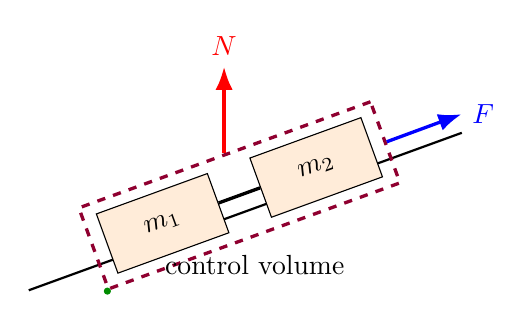
\begin{tikzpicture}[>=Latex]
  \draw[thick] (-.5,-.2) -- (5,1.8);
  \node[draw,fill=orange!15,minimum width=15mm,minimum height=8mm,rotate=20] (m1) at (1.2,.65) {$m_1$};
  \node[draw,fill=orange!15,minimum width=15mm,minimum height=8mm,rotate=20] (m2) at (3.15,1.36) {$m_2$};
  \draw[very thick] (m1.east) -- (m2.west);

  \node[rotate fit=20,fit=(m1)(m2),draw=purple!75!black,dashed,
    line width=1.2pt,inner xsep=5pt,inner ysep=4pt] (system) {};
  \draw[->,very thick,red] (system.north) -- ++(0,1.1) node[above] {$N$};
  \draw[->,very thick,blue] (system.east) -- ++(.95,.35) node[right] {$F$};
  \fill[green!55!black] (system.south west) circle (1.3pt);
  \node[below=3pt] at (system.south) {control volume};
\end{tikzpicture}
\end{document}
